\subsection{Linear models with interactions}\label{sec:linear_model}

%\frame {
%\frametitle{Linear models with interactions}
%\setbeamertemplate{itemize items}[ball]		
%Lasso
%\begin{itemize}
%	\setlength\itemsep{0,5em}
%	\item  Let $y = ( y_1 , y_2 , . . . , y_n )$ 0 denote the vector of responses and let X denote the design matrix. Then the lasso is defined as
%	\end{itemize}			 			 
%\begin{equation}
%\hat{\boldsymbol{\beta}}^{L A S S O}=\arg \min _{\boldsymbol{\beta}}\left(\frac{1}{2}\|\mathbf{y}-\mathbf{X} \boldsymbol{\beta}\|_{2}^{2}+\lambda\|\boldsymbol{\beta}\|_{1}\right)
%\end{equation}
%
%\;\;\;\;\;\;\centering where $\|\cdot\|_{2}$ denotes the $\ell^{2}$ -norm, $\|\cdot\|_{1}$ denotes the $\ell^{1}$ -norm, and $\lambda$ is a tuning parameter that controls the amount of regularization.
%	  
%}
% \begin{block}{Interaction model}
%As mentioned earlier it was proposed different metamodeling approaches to compute the FMV of large VA portfolios.
% table $\#$ summarizes some of the main papers/metamodels dedicated to this task.

%\begin{figure}[h!]
%\makebox[\textwidth][c]{
%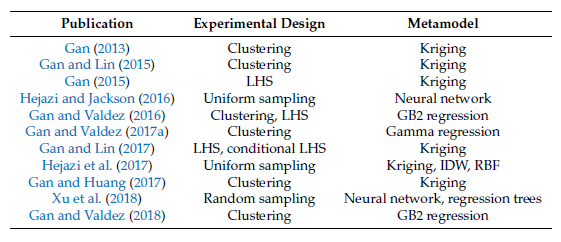
\includegraphics[scale=0.9]{pictures/some_approaches}
%}
%\end{figure}

% \textit{Include here the table 3 of paper: Valuation of large variable annuity portfolios using linear models with interactions}

%A brief look to the table above allow us verify that some approaches are quite sophisticated, e.g. kriging, neural network, GB2 regression. 

In this section, following \cite{gan2018valuation}, 
%it will be presented a linear regression model with interaction effects as an alternative method. 
a linear regression model with interaction effects is used in the valuation of VA contracts.
The main advantages of the approach discussed here is the simplicity in the metamodeling process, 
and the possibility of exploring interactions terms as features to predict the FMV of VA contracts. 

\subsubsection*{Interaction model}

% \vspace{0.25cm}
%By definition, an interaction exists between X and Y in a function $\textit{f}$ when $\textit{f}$ cannot be expressed as $g(x) + h(x)$, in other words, there are interactions when the response variable cannot be explained by additive function of the independent variables.
% \end{block}

By definition, interactions exist in a regression model when the response variable cannot be explained by additive functions of the independent explanatory variables.
%
%
Let $Y$ be a continuous response variable, and let $X_1, X_2, X_3, ..., X_n$ be the explanatory variables, including categorical and continuous, that will be used to model $Y$. The first-order interaction model can be write as:
% \vspace{0.5cm}

% \begin{block}{First order interaction model}
\begin{equation}
Y = \mu+\sum_{i=1}^{p} X_{i} \beta_{i}+\sum_{i<j} X_{i : j} \beta_{i : j} + \varepsilon,
\end{equation}

where the term $X_i$ denotes the individual effect of $X_i$ on $Y$; and $X_{i:j}$ denotes the effect of interaction between $X_i$ and $X_j$ on $Y$. In general lines, the equation (5.1) corresponds to an extension of the multiple linear regression model that is obtained with the inclusion of interaction terms.

The inclusion of interaction terms as explanatory variables can be viewed as the main virtue of the presented approach, since the added variables help to increase the predictive power of the model; however if the number of interaction terms to be included in the regression model is large, the estimated model can overfit the data. To avoid overfitting problem, two shrinkage methods are used to select the relevant interactions and estimate the parameters: group-LASSO and overlapped group-LASSO, to be presented in the next subsection.

% \begin{description}
% \item [$X_i$] main effect matrix
% %\item [$\beta_i$] main effect coefficient
% \item [$X_{i:j} $] interaction matrix
% %\item [$\beta_{i:j}$] main effect coefficient
% \end{description}
% \end{block}

% Types of interaction pairs:
% \begin{itemize}
%  \item categorical variables,
%  \item continuous variables,
%  \item categorical and continuous.
% \end{itemize}

% \begin{block}{Estimation of parameters}
\subsubsection*{Estimation of parameters}

Group-LASSO (GLASSO) and overlapped Group-LASSO (OGLASSO) can be considered general versions of the  LASSO,~\cite{tibshirani1996regression}. While the latter is designed for selecting individual input variables, GLASSO and OGLASSO are able to select important factors, or group of relevant variables.

Suppose that there are \textit{p} groups of variables. For $j = 1, 2, 3, ..., p$, let $\mathbf{X}_j$ denotes the feature matrix for group \textit{j}. The GLASSO can be formulated as:
% By solving the optimization problem
% \begin{equation}
% \hat{\beta}=\arg \min _{\beta} \left(\frac{1}{2}\left\|\mathbf{Y}-\mu \cdot \mathbf{1}-\sum_{i=1}^{p} \mathbf{X}_{i} \beta_{i}+\sum_{i<j} \mathbf{X}_{i : j} \beta_{i : j}\right\|_{2}^{2}\right)
% \end{equation}
% \end{block}
% \vspace{0.25cm}
% \begin{block}{Strong hierarchy}
% \vspace{0.25cm}
% Regularization techniques used to enforce \emph{strong hierarchy}.
% \end{block}
% \begin{block}{Lasso}
% \begin{equation}
% \hat{\boldsymbol{\beta}}^{L A S S O}=\arg \min _{\boldsymbol{\beta}}\left(\frac{1}{2}\|\mathbf{y}-\mathbf{X} \boldsymbol{\beta}\|_{2}^{2}+\lambda\|\boldsymbol{\beta}\|_{1}\right),
% \end{equation}
% %where $\lambda$ controls the amount of regularization.
% \end{block}
% \vspace{0.5cm}
% \begin{block}{Group-Lasso}
\begin{equation}
\hat{\beta}^{G L A S S O}=\arg \min _{\beta}\left(\frac{1}{2}\left\|\mathbf{y}-\beta_{0} \mathbf{1}-\sum_{j=1}^{p} \mathbf{X}_{j} \boldsymbol{\beta}_{j}\right\|_{2}^{2}+\lambda \sum_{j=1}^{p} \gamma_{j}\left\|\boldsymbol{\beta}_{j}\right\|_{1}\right),
\end{equation}
%where $X_{j}$ are feature groups and $\gamma_{j}$ are tuning parameters.
% \end{block}
where $\mathbf{1}$ is a vector of ones, $\left\| \bullet \right\|_2$ denotes the $\ell^{2}$-norm, and $\lambda, \gamma_1, ..., \gamma_p$ are tuning parameters. The parameter $\lambda$ controls the overall amount of regularization while the parameters $\gamma_1, ..., \gamma_p$ allow each group to be penalized to different extents. An attractive property of the GLASSO is that if $\boldsymbol{\hat{\beta_{j}}}$ is nonzero, then all of its components are typically nonzero.

% $\boldsymbol{\beta}$

In an intuitive way, GLASSO gives us the $\boldsymbol{\hat{\beta_j}}$ that minimize the mean squared error given a penalization term that shrinks parameters to zero. The selected group of variables are those related to the parameters that are nonzero. Optimal penalization terms can be chosen by cross-validation.

%\frame {
%\frametitle{Linear models with interactions}
%\setbeamertemplate{itemize items}[ball]		
%Group-Lasso
%\begin{itemize}
%	\setlength\itemsep{0,5em}
%	\item The group-lasso can be viewed as a general version of the popular Lasso.
%	\item Suppose that there are $p$ groups of variables. For $j=1,2, \ldots, p,$ let $X_{j}$ denote the feature matrix for group $j .$ The group-lasso can be formulated as follows:
%\end{itemize}			 			 
%\begin{equation}
%\hat{\beta}^{G L A S S O}=\arg \min _{\beta}\left(\frac{1}{2}\left\|\mathbf{y}-\beta_{0} \mathbf{1}-\sum_{j=1}^{p} \mathbf{X}_{j} \boldsymbol{\beta}_{j}\right\|_{2}^{2}+\lambda \sum_{j=1}^{p} %\gamma_{j}\left\|\boldsymbol{\beta}_{j}\right\|_{2}\right)
%\end{equation}
%
%\;\;\;\;\;\;\centering where 1 is a vector of ones, $\|\cdot\|_{2}$ denotes the $\ell^{2}$ -norm, and $\lambda, \gamma_{1}, \ldots, \gamma_{p}$ are tuning parameters.
%	  
%}

% \begin{block}{Overlapped Group-Lasso}
% \vspace{0.15cm}
% Group-Lasso with variables that can show up in different groups.
% \end{block}

The OGLASSO extends the GLASSO by adding an overlapped Group-LASSO penalty to the loss function in order to obtain hierarchical interaction models that can be formulated as the following unconstrained optimization problem:

% \begin{align*}
% \hat{\beta}^{O G L A S S O} &=\arg \min _{\beta}\left(\frac{1}{2}\left\|\mathbf{y}-\beta_{0} \mathbf{1}-\Sigma_{j=1}^{p} \mathbf{X}_{j} \beta_{j}-\sum_{s<t} \boldsymbol{X}_{s : t} \boldsymbol{\beta}_{s : t}\right\|_{2}^{2}\right. \\
% &+\lambda\left(\sum_{j=1}^{p}\left\|\boldsymbol{\beta}_{j}\right\|_{2}+\sum_{s<t}\left\|\boldsymbol{\beta}_{s : t}\right\|_{2}\right)\right)
% \end{align*}

\begin{align*}
\hat{\beta}^{O G L A S S O} =\arg \min _{\beta}\left(\frac{1}{2}\left\|\mathbf{y}-\beta_{0} \mathbf{1}-\Sigma_{j=1}^{p} \mathbf{X}_{j} \beta_{j}-\sum_{s<t} \boldsymbol{X}_{s : t} \boldsymbol{\beta}_{s : t}\right\|_{2}^{2}\\
\left +\lambda\left(\sum_{j=1}^{p}\left\|\boldsymbol{\beta}_{j}\right\|_{1}+\sum_{s<t}\left\|\boldsymbol{\beta}_{s : t}\right\|_{1}\right)\right)
\end{align*}

Unlike the GLASSO, the OGLASSO is capable of selecting interactions between groups as relevant explanatory variables.
%\frame {
%\frametitle{Linear models with interactions}
%\setbeamertemplate{itemize items}[ball]	
%Overlapped Group-Lasso
%\begin{figure}%
%	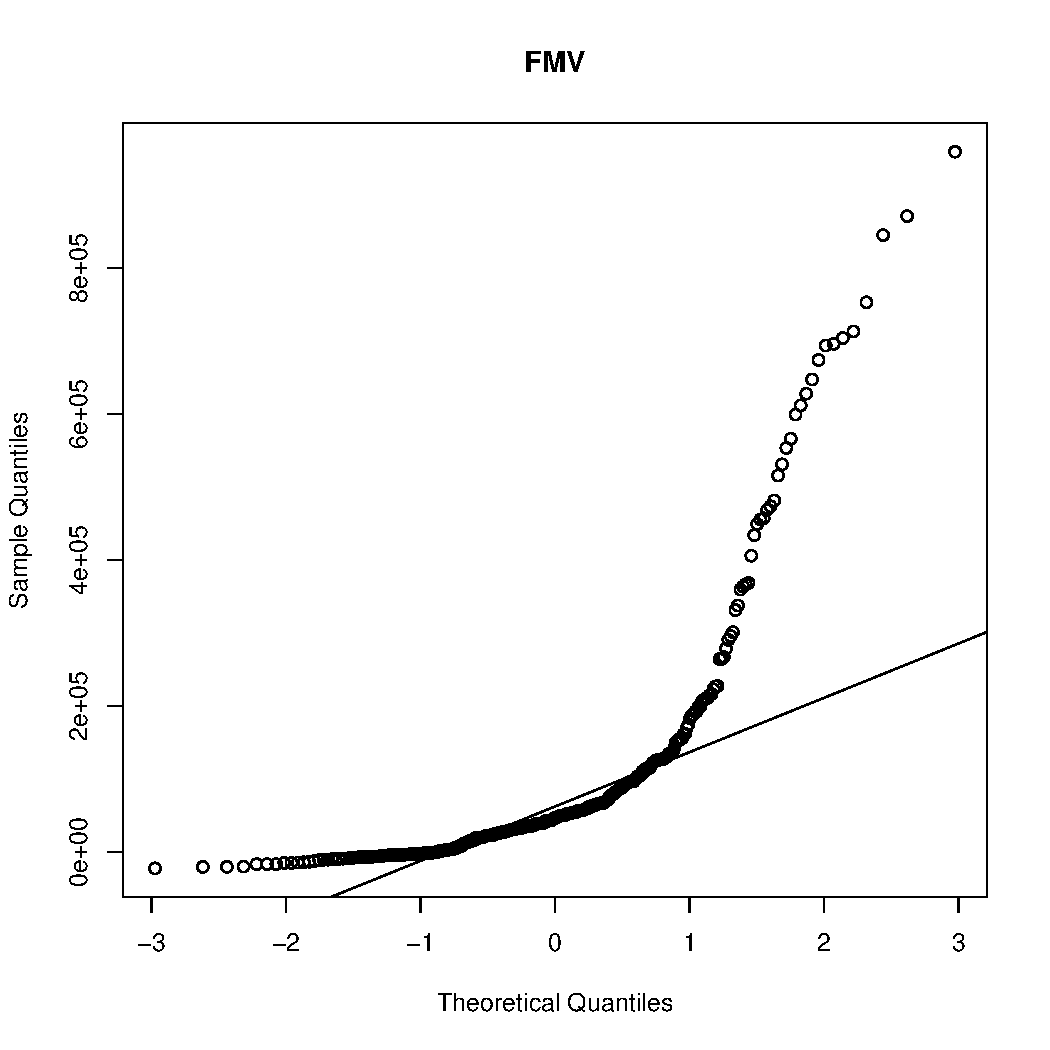
\includegraphics[width=0.6\linewidth]{figure5.pdf}
%	\caption{Overlapped Group-Lasso}
%\end{figure}
%}
\subsubsection*{Empirical results}\label{empirical_results}

The following results were computed for two independent representative portfolios of VA contracts, extracted from the synthetic data set described in Chapter~\ref{chap:dataset}. For each of them, a linear model with interactions was estimated based on the OGLASSO. The plots in Figure~\ref{original_fmv} show histograms of the FMVs as a preliminary examination of the target variable. As illustrated, the distribution is skewed to the right and there are many contracts with FMV close to zero. The QQ-plots in Figure~\ref{original_fmv} compare the theoretical distribution of the FMV (Normal) with its empirical distribution. Based on the graphical analysis it is possible to assert that the FMVs do not follow a Normal distribution, as many points on the plot are located far away from the straight line.

\begin{figure}[h!]
\makebox[\textwidth][c]{
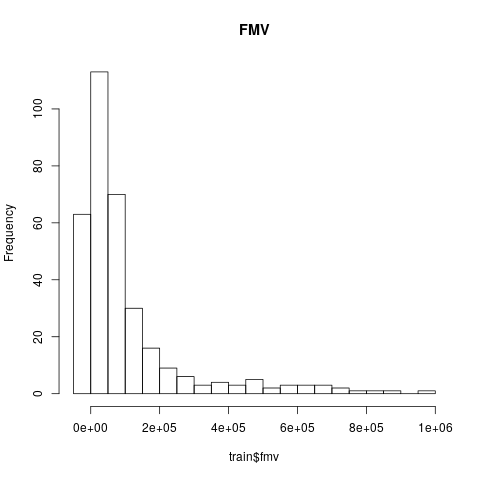
\includegraphics[scale=0.4]{pictures/original_fmv_hist_rep1}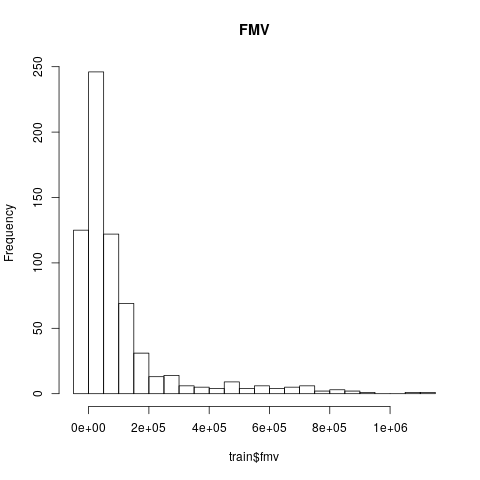
\includegraphics[scale=0.4]{pictures/original_fmv_hist_rep2} 
}
\makebox[\textwidth][c]{
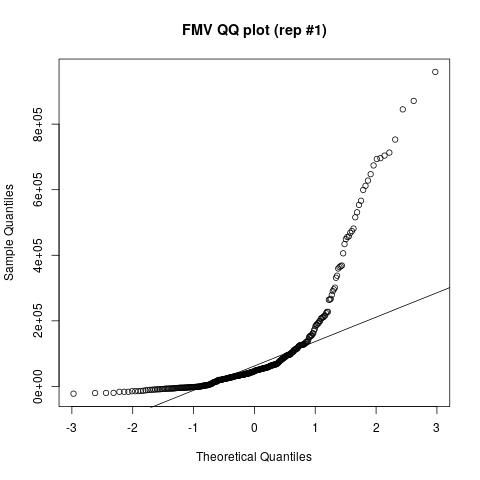
\includegraphics[scale=0.4]{pictures/boxcox_rep1_fmv_qqplot}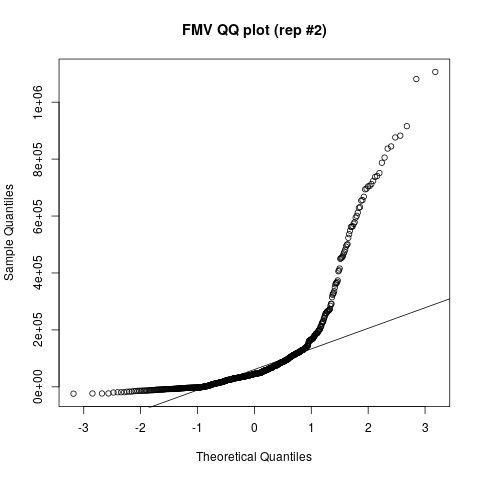
\includegraphics[scale=0.4]{pictures/boxcox_rep2_fmv_qqplot} 
}
\caption{Histograms and QQ-plots for the fair market values of the contracts in the representative portfolios.}\label{original_fmv}
\end{figure}

%After estimating the model parameters for both representative portfolios, we verify the gaussianity of the residuals. First, their histograms are illustrated in Figure~\ref{histogram_residuals_fmv}.

\begin{figure}[h!]
\makebox[\textwidth][c]{
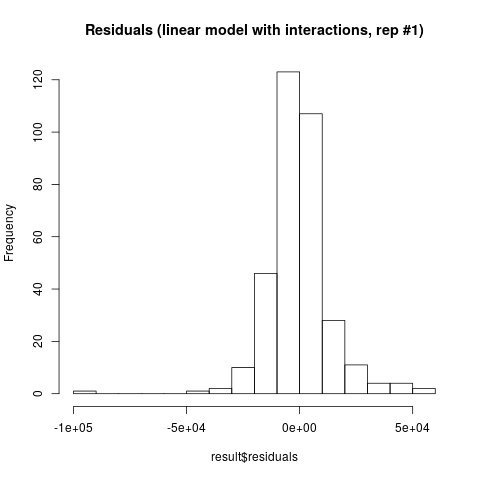
\includegraphics[scale=0.4]{pictures/original_residuals_linear_model_with_interactions_hist_rep1}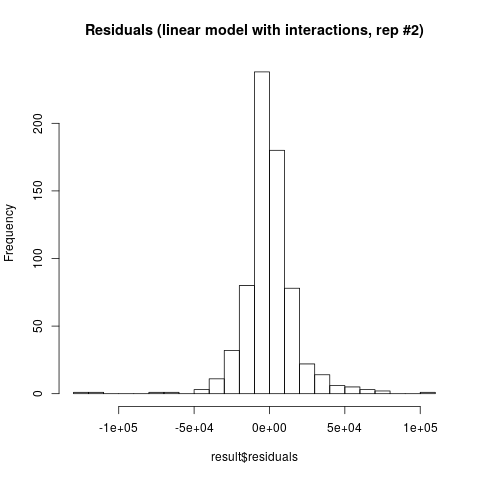
\includegraphics[scale=0.4]{pictures/original_residuals_linear_model_with_interactions_hist_rep2} 
}
\makebox[\textwidth][c]{
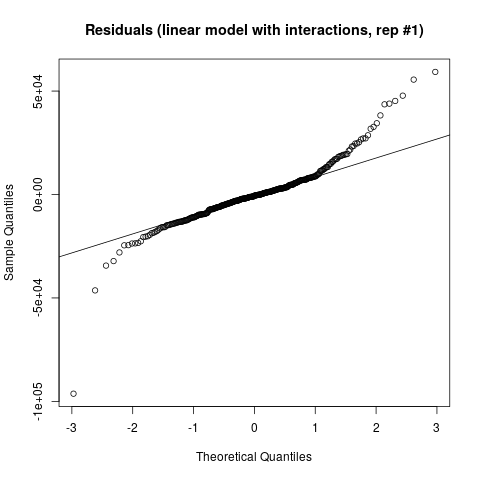
\includegraphics[scale=0.4]{pictures/original_residuals_linear_model_with_interactions_qqplot_rep1}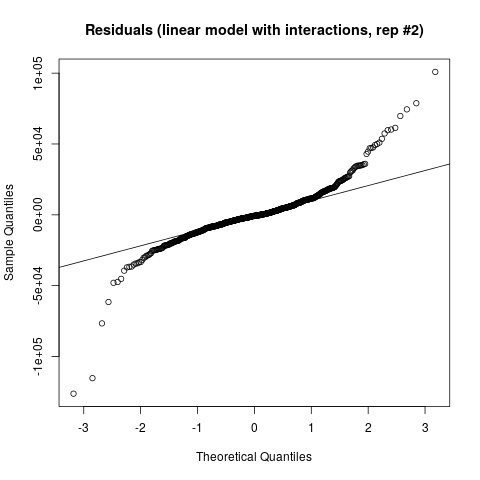
\includegraphics[scale=0.4]{pictures/original_residuals_linear_model_with_interactions_qqplot_rep2} 
}
%\caption{QQ-plots for the regression residuals for the OGLASSO models}\label{qq_plot_residuals_fmv}
\caption{Histograms and QQ-plots for the residuals of the OGLASSO models fitted for each representative portfolio.}\label{residuals_oglasso}
\end{figure}

After estimating the model parameters for both representative portfolios, we analyse the residuals of the OGLASSO models. Histograms and QQ-plots are shown in Figure~\ref{residuals_oglasso}. As expected, the residuals illustrated in the histograms are centered around zero. In addition, as the QQ-plots indicate, the residuals present heavy tails, a feature that is not consistent with the hypothesis of a Normal distribution. 
%
%The two first histograms above show the distribution of residuals after fitting the OGLASSO model, while the following two show the QQ-plot of residuals, taking the standard normal as theoretical distribution. Residuals distributed as a standard normal is a desirable property, since it is a necessary assumption to make valid inference on the estimated parameters.
%
Normally distributed residuals are a desirable feature to validate any inference built on top of the estimated parameters. As illustrated in Figure~\ref{interactions}, the statistically significant interaction terms identified for each representative portfolio are quite different.

%As residuals are clearly non-gaussian, the inference on the model is not consistent, as shown in Figure~\ref{interactions} where the significant interaction terms are illustrated.

\begin{figure}[h!]
\makebox[\textwidth][c]{
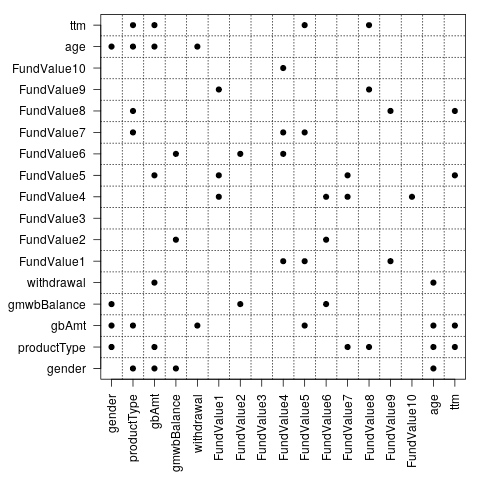
\includegraphics[scale=0.4]{pictures/original_interactions_model_rep1}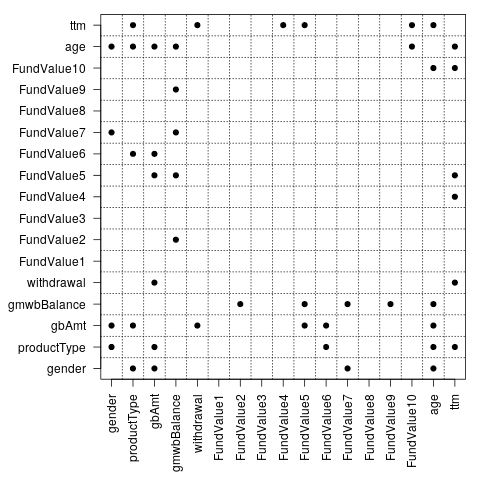
\includegraphics[scale=0.4]{pictures/original_interactions_model_rep2} 
}
\caption{Interaction matrices for the OGLASSO models, showing the statistically significant interaction terms in each model.}\label{interactions}
\end{figure}

%Analysing the last graphs, we can observe that there are some values in the tail of empirical distribution that are not fitted by a standard normal, consequently inference on the model is not consistent. 

%Despite the fact, the results show that the model is able to make good predictions of the FMV.

Despite the problems identified in the residuals of the fitted models, their predictions are quite satisfactory. These are illustrated using the QQ-plots in Figure~\ref{prediction_fmv}, where predicted FMVs are compared against their correct values. The in-sample results, computed exclusively with the contracts in the representative portfolios, give us $R^2$ values equal to 0.9928 and 0.9891 for each representative portfolio. For the full data set of VA contracts, $R^2$ values are equal to 0.9526 and 0.9618.

%The graphs above compare the model predictions for the training set and the true FMV. As closer the points are to the straight line as better is the fit in sample. 

\begin{figure}[h!]
\makebox[\textwidth][c]{
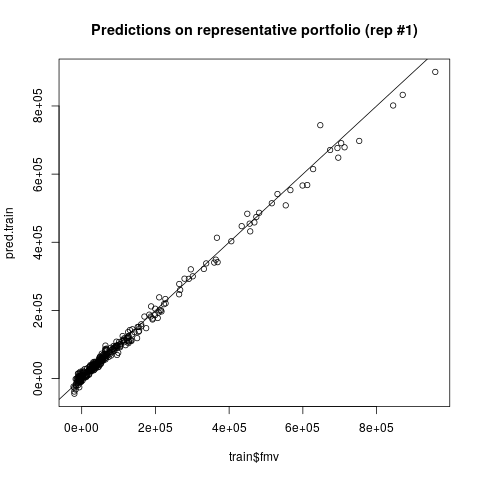
\includegraphics[scale=0.4]{pictures/original_predictions_representative_portfolio_rep1}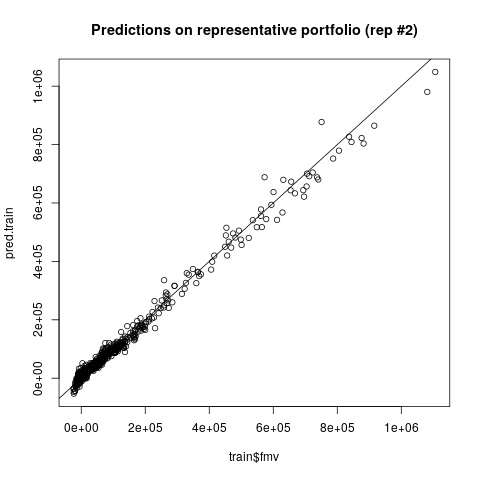
\includegraphics[scale=0.4]{pictures/original_predictions_representative_portfolio_rep2} 
}
\makebox[\textwidth][c]{
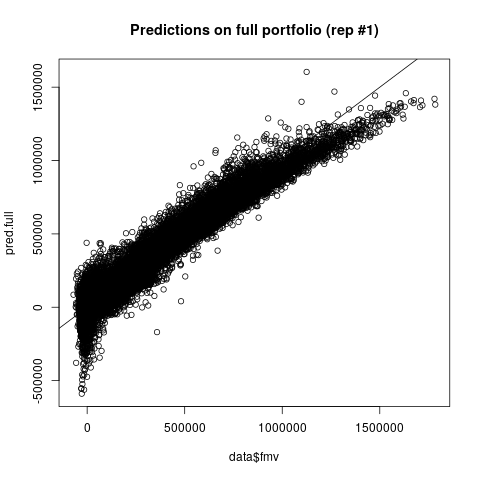
\includegraphics[scale=0.4]{pictures/original_predictions_full_portfolio_rep1}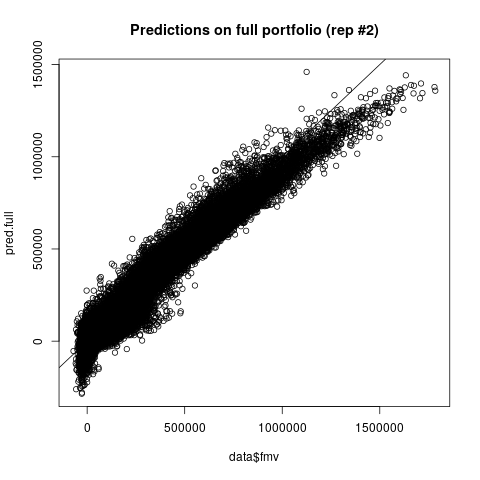
\includegraphics[scale=0.4]{pictures/original_predictions_full_portfolio_rep2} 
}
\caption{In-sample (representative portfolio) and out-of-sample (full portfolio) analysis of the predicted fair market values for VA contracts}\label{prediction_fmv}
\end{figure}

%The graphs above compare the model predictions for the training set and the true FMV. As closer the points are to the straight line as better is the fit in sample. The $r^2$ for each representative set are 0.9928 and 0.9891, respectively.
%Considering the remaining data for each representative set, the $r^2$ obtained are 0.9526 and 0.9618, respectively. The graphs bellow show the results.

% \begin{center}
% True FMV versus model predictions (training set)\\
% $r^2$: $0.9928$ and $0.9891$
% \end{center}

%In summary, the numeric results presented above show that including interaction in linear regression models is an interesting strategy to improve predictions of FMV and metamodeling process. However, as an important assumption is violated, inference based on the estimated parameters is inconsistent. In the next section, it will be discussed a transformation technique to enable consistent estimation and interpretation of parameters.

In summary, as expected, the numeric results presented above confirm that linear models with interaction terms provide excellent results for the valuation of portfolios of VA contracts. However, as an important assumption is violated, inference based on the estimated parameters is inconsistent, as illustrated in Figure~\ref{interactions}. In the next section, we discuss a technique that improves the consistency of the results.

% \begin{center}
% True FMV versus model predictions (all data)\\
% $r^2$: $0.9526$ and $0.9618$
% \end{center}

% \begin{center}
% An example with two representative portfolios:
% \end{center}

% \begin{center}
% Interactions are inconsistent!
% \end{center}

